\documentclass[12pt]{article}
\makeatletter
\newcommand*{\rom}[1]{\expandafter\@slowromancap\romannumeral #1@}
\makeatother
\usepackage{amsfonts, amssymb}
\usepackage{mathrsfs, mathdots} 
\usepackage{amsmath}
\usepackage{float}
\usepackage{amsthm}
\usepackage{tikz-cd}
\usepackage{xcolor}
\usepackage{xparse}
\usepackage{setspace}
\usepackage{xfrac}
\usepackage{yfonts}

\newtheorem{theorem}{Theorem}[subsection]
\newtheorem{proposition}[theorem]{Proposition}
\newtheorem{corollary}[theorem]{Corollary}
\newtheorem{lemma}[theorem]{Lemma}
\newtheorem{notations}[theorem]{Notations}
\newtheorem{definition}[theorem]{Definition}
\newtheorem{example}[theorem]{Example}

\ExplSyntaxOn
\NewDocumentCommand{\cycle}{ O{\;} m }
 {
  (
  \alec_cycle:nn { #1 } { #2 }
  )
 }

\seq_new:N \l_alec_cycle_seq
\cs_new_protected:Npn \alec_cycle:nn #1 #2
 {
  \seq_set_split:Nnn \l_alec_cycle_seq { , } { #2 }
  \seq_use:Nn \l_alec_cycle_seq { #1 }
 }
\ExplSyntaxOff
\usepackage{titling}
\newcommand{\subtitle}[1]{%
  \posttitle{%
    \par\end{center}
    \begin{center}\large#1\end{center}
    \vskip0.5em}%
}
\usepackage{arydshln}
\setcounter{tocdepth}{2}
\setlength{\dashlinedash}{1.2pt}
\setlength{\dashlinegap}{1.5pt}
\setlength{\arrayrulewidth}{0.2pt}
\begin{document}
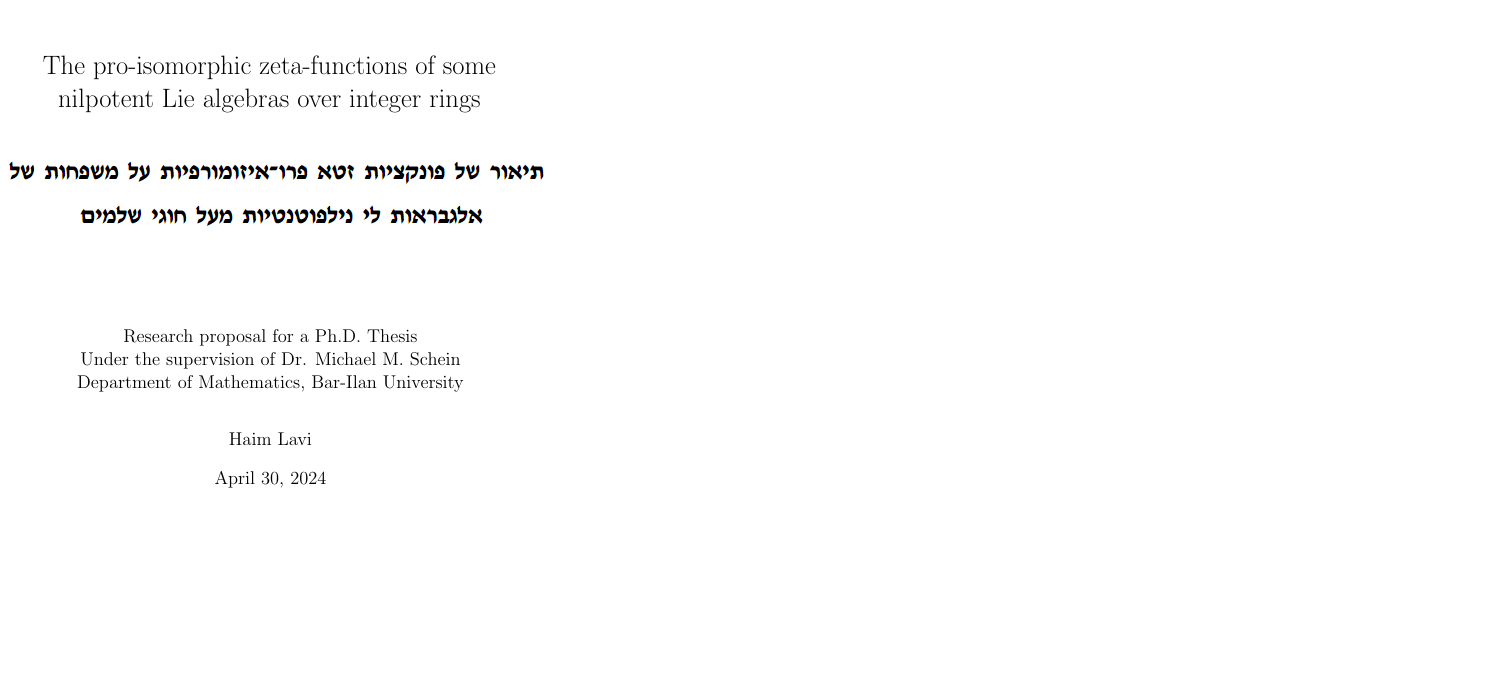
\includegraphics{title}
\newpage
\tableofcontents
\newpage
\begin{abstract}
Let $G$ be any group. For any natural number $n\in\mathbb{N}$, let $a_n$ be the number of subgroups $H\leq G$, such that $[G:H]=n$. Assume $G$ is finitely-generated, then $a_n<\infty$, and we can define a Dirichlet series of the form $\zeta_G(s):=\sum_{n=1}^\infty a_n n^{-s}$, where $s\in\mathbb{C}$. Assume, in addition, that $G$ is also nilpotent and torsion-free, then this function has some properties of the Riemann $\zeta$-function, such as the Euler decomposition of $\zeta$ into a product of local factors indexed by primes. A version of this $\zeta$-function counts pro-isomorphic subgroups, and an analogous function may be defined for appropriate Lie rings. We study here the pro-isomorphic $\zeta$-functions for a family of nilpotent Lie rings of unbounded nilpotency class. We shall compute the automorphism groups of these Lie rings explicitly, prove uniformity of the local factors of the pro-isomorphic $\zeta$-functions, and aim to determine them explicitly.
\end{abstract}
\section{Scientific Background}
\subsection{Introduction}
We start our discussion with the following proposition, which stands at the very foundation of our subject.
\begin{proposition} \label{prop:finite.number.subgroups}
Let $G$ be any finitely generated group, and let $n\in\mathbb{N}$ be any natural number. Then there is a finite number of subgroups $H\leq G$, such that $[G:H]=n$
\end{proposition}
\begin{proof}
Let $H\leq G$ be a subgroup, such that $[G:H]=n$, and let $\sfrac{G}{H}:=\{g_1H,g_2H,\dots,g_nH\}$ be the set containing all left-cosets of $H$ in $G$. We may consider the action of $G$ by left multiplication on $\sfrac{G}{H}$: for all $g\in G$, and for all left-cosets $g_iH\in\sfrac{G}{H}$, we have that $g(g_iH):=(gg_i)H=g_jH$, where $g_jH\in\sfrac{G}{H}$ is some left-coset. This means that $g$ maps every index $i\in[n]$ to some index $j\in[n]$, which means that $g$ operates as a permutation on $[n]$. Therefore, there exists a homomorphism $f:G\rightarrow\mathcal{S}_n$, from $G$ to the symmetric group of order $n$. Let $1\leq k\leq n$ be the index for which $g_kH=H$. For all $g\in G$, $g\in H$ if and only if $gH=H$, which means that $(gg_k)H=g(g_kH)=gH=H=g_kH$, which means that $f(g)(k)=k$, in words, $k$ is fixed by the image $f(g)$. This means that $H=\{g\in G : f(g)(k)=k\}$, so $H$ may be recovered from the homomorphism $f$, which clearly shows that the number of subgroups $H\leq G$ of index $n$ is less or equal to the number of maps $f : G
\rightarrow\mathcal{S}_n$. We assumed that $G$ is finitely-generated, and $\mathcal{S}_n$ is obviously finite. We know that group homomorphisms are uniquely determined by the maps of their generators. Therefore, there are finitely many maps from a finite set of generators to a finite group, which clearly shows that the number of subgroups $H\leq G$ of index $n$ is necessarily finite.
\end{proof}
This proposition gives rise to an entire subject in group theory, called \textbf{subgroup growth}. We denote by $a_n(G)$ the number of subgroups of $G$ of index $n$, and look at the sequence $\{a_n(G)\}_{n=1}^{\infty}$. The subject of subgroup growth aims to relate the properties of this sequence to the algebraic structure of $G$. For instance, Lubotzky, Mann and Segal showed in \cite{LubotzkyMannSegal} that $a_n(G)$ grows polynomially if and only if $G$ is virtually solvable of finite rank, that is, $G$ has a finite-index solvable subgroup, and all finitely-generated subgroups may be generated by a bounded number of generators. This research concentrates on the growth of \textbf{pro-isomorphic} subgroups, which we now define.
\begin{definition}
\label{def:profinite.closure}
Let $G$ be any group, and let $\mathcal{N}(G):=\{N_k\trianglelefteq G\}_{k\in I}$ be the set of all normal subgroups of $G$. We define a partial order on $\mathcal{N}(G)$ by reverse inclusion, that is for every two indices $i,j$ we say that $i\leq j$ if and only if $N_j\subseteq N_i$, hence for every $i\leq j$ there exists a natural projection map $\pi_{ji}:\sfrac{G}{N_
j}\rightarrow\sfrac{G}{N_i}$. The inverse limit \[\widehat{G}=\underset{\leftarrow}{lim}\{\sfrac{G}{N_k}\}_{k\in I}:=\{(h_k)_{k\in I}\in\prod_{k\in I}\sfrac{G}{N_k} : \pi_{ji}(h_j)=h_i,\forall i\leq j\}\] is called the \textbf{profinite closure} of $G$.
\end{definition}
\begin{definition}
\label{def:pro.isomorphic}
Let $G$ be any group. A subgroup $H\leq G$ is called \textbf{pro-isomorphic} if $\widehat{H}\cong\widehat{G}$.
\end{definition}
\begin{definition}
\label{def:zeta.pro.isomorphic}
Let $G$ be any group, and let \[\hat{a_n}(G):=\#\{H\leq G : \widehat{H}\cong\widehat{G}, [G:H]=n\}\] be the number of pro-isomorphic subgroups of $G$ of index $n$. Assume that $\hat{a_n}(G)<\infty$ for all $n$. The \textbf{pro-isomorphic $\zeta$-function} of $G$ is defined by $\hat{\zeta_G}(s):=\sum_{n=1}^{\infty}\hat{a_n}(G)n^{-s}$ for $s\in\mathbb{C}$.
\end{definition}
If our $\zeta$-function, which is a special case of the Dirichlet series, has some properties of convergence on some subset of $\mathbb{C}$, one may reconstruct its coefficients $\hat{a_n}(G)$, which, in our case, are the number of subgroups of our interest, using the \textbf{Perron's forumla}, which is an implementation of a \textbf{reverse Mellin transform}, as discussed, for example, in \cite{MontgomeryVaughan}. This method, including the specific properties of convergence required for the reconstruction, is out of the scope of our research, and therefore will not be further discussed, at this stage.\par
It is known that if $\hat{a_n}(G)$ grows polynomially, then $\hat{\zeta_G}(s)$ converges on some right half-plane of $\mathbb{C}$. For instance, we take the group $G=(\mathbb{Z},+)$. The group $\mathbb{Z}$ is an abelian group, and every subgroup is of the form $H=n\mathbb{Z}=\langle n\rangle$, for some $n\in\mathbb{N}$, which means that $H\cong \mathbb{Z}$, as both are infinite cyclic groups, and so, $\widehat{H}\cong\widehat{\mathbb{Z}}$. Since we have only one subgroup of index $n$, for every $n\in\mathbb{N}$, then $a_n(\mathbb{Z})=\hat{a_n}(\mathbb{Z})=1$. Thus, its pro-isomorphic $\zeta$-function is $\hat{\zeta_{\mathbb{Z}}}=\sum_{i=1}^{\infty}n^{-s}=\zeta(s)$, the Riemann $\zeta$-function, which is known to converge for $Re(s)>1$.\par
After establishing the basic definitions, we observe a fact that is a major motivation for this research, which says that the Riemann $\zeta$-function decomposes into an infinite product of local zeta-functions, that is, $\zeta(s)=\prod_p\zeta_p(s)=\prod_p\sum_{k=0}^\infty p^{-ks}=\prod_p\frac{1}{1-p^{-s}}$, where the product runs over all the prime numbers. Following this fact regarding the Riemann $\zeta$-function, we observe that for any finitely-generated, nilpotent and torsion-free group $G$, we have the same decomposition as above for the pro-isomorphic $\zeta$-function: $\hat{\zeta_G}(s)=\prod_p\hat{\zeta_{G,p}}(s)$, where $\hat{\zeta_{G,p}}(s):=\sum_{k=0}^\infty \hat{a_{p^k}}(G)p^{-ks}$. The general construction of $\zeta$-functions, as well as their Euler decomposition to local zeta-functions, for the study of subgroup growth, were well established by Grunewald, Segal and Smith, in \cite{GrunewaldSegalSmith}. We hereby bring several basic definitions of group nilpotency, which are very important for this research.
\begin{definition}
\label{def.lower.central.series}
Let $G$ be any group. The \textbf{lower central series} of $G$ is a sequence of subgroups of $G$ defined by the recursive rule $G_k:=[G,G_{k-1}]$, for every $k\in\mathbb{N}$, where $G_0:=G$.  We recall that $[G,G_k]\leq G$ is the subgroup generated by the collection of commutators $\{gg_kg^{-1}g_k^{-1} : g\in G,g_k\in G_k\}$.
\end{definition}
\begin{definition}
\label{def.nilpotency.class}
Let $G$ be any group. The \textbf{nilpotency class} of $G$ is $min\{k\in\mathbb{N} : G_k=[G,G_{k-1}]=\{e\}\}$, in words, the smallest natural number $k$, such that the subgroup of commutators of the form $[G,G_{k-1}]$ is the trivial group. We can extend this definition, and say that the trivial group nilpotency class is $0$.
\end{definition}
\begin{definition}
\label{def.nilpotent.group}
Let $G$ be a group. If $G$ is of finite nilpotency class, then $G$ is said to be a \textbf{nilpotent} group.
\end{definition}
\subsection{Linearization}
We want to transfer the ideas from the above discussion about groups to a linear context, where we can use tools from linear algebra.
Hence, for finitely-generated torsion-free nilpotent groups $G$, we associate nilpotent Lie algebras over $\mathbb{Z}$. This, in general, is called the \textbf{Maltsev correspondance}. 
If $L$ is a $\mathbb{Z}$-Lie algebra, namely a free $\mathbb{Z}$-module of finite rank with a Lie brackets operation, then consider the (finite) number $\hat{a_n}(L)$ of subalgebras $M\leq L$, such that $M\otimes\mathbb{Z}_p\cong L\otimes\mathbb{Z}_p$ for all primes $p$. The Dirichlet series $\hat{\zeta_L}(s):=\sum_{n=1}^{\infty}\hat{a_n}(L)n^{-s}$, is called the \textbf{pro-isomorphic zeta-function} of $L$. By the Maltsev correspondence, to every finitely-generated, nilpotent, torsion-free group $G$, one may associate a Lie algebra $L(G)$, such that $\hat{\zeta_{G,p}}(s)=\hat{\zeta_{L,p}}(s)$, for but finitely many primes $p$. If $G$ has nilpotency class $2$, one may obtain the equality for all primes. Let $n\in\mathbb{N}$, and let $L_n$ be a $\mathbb{Z}$-Lie algebra, and fix a $\mathbb{Z}$-basis $\mathcal{B}=\{b_1,\dots,b_r\}$, where $r$=rank$L_n$ depends on $n$. Let $\mathcal{L}_{n,p}=L_n\otimes_{\mathbb{Z}}\mathbb{Q}_p$, for any $p$. This is a $\mathbb{Q}_p$-Lie algebra, and our choice of basis allows us to identify the automorphism group $G_n(\mathbb{Q}_p)=Aut_{\mathbb{Q}_p}(\mathcal{L}_{n,p})$ with a subgroup of $GL_r(\mathbb{Q}_p)$. Note that $\mathcal{L}_{n,p}$ contains a $\mathbb{Z}_p$-lattice, $L_{n,p}=L_n\otimes_{\mathbb{Z}}\mathbb{Z}_p$. If $\varphi\in G_n(\mathbb{Q}_p)$, then $\varphi(L_{n,p})=L_{n,p}$ if and only if $\varphi\in G_n(\mathbb{Z}_p)=G_n(\mathbb{Q}_p)\cap GL_r(\mathbb{Z}_p)$. Here $GL_r(\mathbb{Z}_p)$ is the group of $r\times r$ matrices which are invertible over $\mathbb{Z}_p$. Similarly, $\varphi(L_{n,p})\subseteq L_{n,p}$ if and only if $\varphi\in G^+_n(\mathbb{Q}_p):=G_n(\mathbb{Q}_p)\cap \mathcal{M}_r(\mathbb{Z}_p)$, where $\mathcal{M}_r(\mathbb{Z}_p)$ is the collection of $r\times r$ matrices with entries in $\mathbb{Z}_p$. Note that $G^+_n(\mathbb{Q}_p)$ is a monoid, not a group.\par
Denote by $G_n(\mathbb{Z}_p)g$, where $g\in G^+_n(\mathbb{Q}_p)$, a right-coset of $G_n(\mathbb{Z}_p)$. One checks that the monoid $G^+_n(\mathbb{Q}_p)$ is a disjoint union of right-cosets of $G_n(\mathbb{Z}_p)$.\par
The discussion above reveals the construction we base our research upon.
We observe that there is a bijection between the set $G_n(\mathbb{Z}_p)\backslash G^+_n(\mathbb{Q}_p)$ of right-cosets of $G_n(\mathbb{Z}_p)$ and the set $\{M\leq L_{n,p} : M\cong L_{n,p}\}$ of $L_{n,p}$-subalgebras which are isomorphic to $L_{n,p}$ itself. This bijection takes $G_n(\mathbb{Z}_p)g$ to $M=\varphi(L_{n,p})$. For any $\varphi\in G_n(\mathbb{Z}_p)g$, this is well-defined. One checks that for every $\psi\in G_n(\mathbb{Z}_p)g$, we have that $\psi(L_{n,p})=\varphi(L_{n,p})=M$.
We end this part, as a preparation for the final part of this technical background review, with the following result, which states that for each right-coset $G_n(\mathbb{Z}_p)g$, if $M=\varphi(L_{n,p})$, where $\varphi\in G_n(\mathbb{Z}_p)g$, then $[L_{n,p}:M]=|\det\varphi|_p^{-1}$, and therefore,\par $\hat{\zeta_{L,p}}(s)=\underset{\overset{\scriptscriptstyle M\leq L_{n,p}}{\scriptscriptstyle M\cong L_{n,p}}}{\sum}[L_{n,p}:M]^{-s}=\underset{\scriptscriptstyle G_n(\mathbb{Z}_p)\varphi\in G_n(\mathbb{Z}_p)\backslash G^+_n(\mathbb{Q}_p)}{\sum}|\det\varphi|_p^s$.
Last for this section, we shall define the lower central series for Lie algebras, which will be our main working tool in the research of the automorphism groups.
\begin{definition}
Let $L$ be a Lie algebra, then the $\textbf{lower central series}$ of $L$ is defined by $\gamma_k L:=[L,\gamma_{k-1}L]$ where $k\in\mathbb{N}$, and $\gamma_1 L:=L$, same as defined for groups in \ref{def.lower.central.series}. A Lie algebra is said to be \textbf{nilpotent}, if $\gamma_k L=\{0\}$, for some finite $k$, also as defined above for groups in \ref{def.nilpotent.group}.
\end{definition}
When the algebra is clear from the context, we may omit the notation of the algebra in $\gamma_k L$, only to stay with the gamma notation $\gamma_k$. Sometimes, we will also use the gamma notation for nilpotnecy classes of groups.
\subsection{$p$-adic Integration}
In this final part of the technical background review, we finally get to the motivation for all the construction we have presented in the first parts. We now define a very central object for our research. We shall assume, without proof, the existence of such an object, under the prerequisites of the definition.
\begin{definition}
\label{def.right.haar.measure}
Let $\Gamma$ be a locally compact topological group, i.e. for all $\gamma\in\Gamma$, there is an open neighborhood of $\gamma\in U_{\gamma}$ and a compact subset $K_{\gamma}$, such that $U_{\gamma}\subset K_{\gamma}$. Then there is a measure $\mu$, with the following property: for any measurable subset $U\subseteq\Gamma$ and any $\gamma\in\Gamma$, $\mu(U\gamma)=\mu(U)$, where $U\gamma:=\{u\gamma : u\in U\}$. Such a measure $\mu$ is called a \textbf{right Haar measure}, and is unique up to multiplication by a non-zero constant.
\end{definition}
Equipped with the right Haar measure, we can finally make use of the construction from above. We start by claiming, without proof, that for every prime number $p$, the group $G_n(\mathbb{Q}_p)$ is a locally compact topological group. We also claim that the right Haar measure has the property that $\mu(G_n(\mathbb{Z}_p))=1$. The measure of all the right-cosets of $G_n(\mathbb{Z}_p)$ equals to the measure of $G_n(\mathbb{Z}_p)$ itself, i.e. for every $g\in G^+_n(\mathbb{Q}_p)$, we have that $\mu(G_n(\mathbb{Z}_p)g)=\mu(G_n(\mathbb{Z}_p))=1$.
With this observation, we go directly to the calculation of the $p$-adic norm of the determinant of every $L_{n,p}$-automorphism, as a $p$-adic integral over our measure space.
First, we observe that given any $L_{n,p}$-automorphism in some right-coset $\varphi\in G_n(\mathbb{Z}_p)\varphi$, we have that $|\det\varphi|_p^s=\displaystyle\int_{G_n(\mathbb{Z}_p)\varphi}|\det\varphi|_p^sd\mu$, because $\mu(G_n(\mathbb{Z}_p)\varphi)=1$, and $|\det\varphi|_p^{-1}$ is fixed on $G_n(\mathbb{Z}_p)\varphi$.\par
Going back to our desired function, we observe that\par $\hat{\zeta_{L,p}}(s)=\underset{\scriptscriptstyle G_n(\mathbb{Z}_p)\varphi\in G_n(\mathbb{Z}_p)\backslash G^+_n(\mathbb{Q}_p)}{\sum}|\det\varphi|_p^s=\underset{\scriptscriptstyle G_n(\mathbb{Z}_p)\varphi\in G_n(\mathbb{Z}_p)\backslash G^+_n(\mathbb{Q}_p)}{\sum}\displaystyle\int_{G_n(\mathbb{Z}_p)\varphi}|\det\varphi|_p^sd\mu=\displaystyle\int_{G^+_n(\mathbb{Z}_p)}|\det\varphi|_p^sd\mu$.\par 
This calculation of the local $\zeta_p$-function as a $p$-adic integral was established by the work of du Sautoy and Lubotzky, in \cite{DuSautoyLubotzky}.
This integral is the main object we shall study in this research.
We end this part, of the technical background review, by a theorem and a couple of definitions, which stand in the center of our research goals.
\begin{theorem}
\label{thm.rational.function}
Let $p$ be a prime number, and let $s\in\mathbb{C}$, then $\hat{\zeta_{L,p}}(s)$ is rational, i.e. there is a rational function in one variable $W_p\in\mathbb{Q}(X)$ such that $\zeta_{L,p}(s)=W_p(p^{-s})$.
\end{theorem}
\begin{definition}
\label{def.uniform}
Let $L$ be a $\mathbb{Z}$-Lie algebra, and let $s\in\mathbb{C}$. Then $\hat{\zeta_L}(s)$ is called \textbf{uniform}, if there exists a rational function in two variables $W\in\mathbb{Q}(X,Y)$ such that for every prime number $p$, the local function $\zeta_{L,p}(s)=W(p,p^{-s})$, which means that $\zeta_{L,p}(s)$ has exactly the same form for all primes, since its value depends only on $p$ and $p^{-s}$.
\end{definition}
\begin{definition}
\label{def.finitely.uniform}
Let $L$ be a $\mathbb{Z}$-Lie algebra, and let $s\in\mathbb{C}$. Then $\hat{\zeta_L}(s)$ is called \textbf{ finitely uniform}, if there exists a finite set of rational function in two variables $W_1,W_2,\dots,W_m\in\mathbb{Q}(X,Y)$ such that for every prime number $p$, the local function $\zeta_{L,p}(s)=W_k(p,p^{-s})$, for some $1\leq k\leq m$. One observes immediately that this is a weaker condition on $L$, because a uniform zeta-function is simply a finitely uniform function where $m=1$.
\end{definition}
The theorem ensures that for any $\mathbb{Z}$-Lie algebra, all the local pro-isomorphic zeta-functions are rational functions in $p^{-s}$, but their form can vary between different primes. If we can prove uniformity, for some specific $\mathbb{Z}$-Lie algebra $L$, it means that all its local zeta-functions have exactly the same form as a rational function in $p$ and $p^{-s}$, and if we can prove finite uniformity, then we can at least show that all the local zeta-functions have only a finite number of different forms.
The uniformity is also established in the work of Grunewald, Segal and Smith, see \cite{GrunewaldSegalSmith}.
Proving the uniformity of the pro-isomorphic zeta-functions of the algebras we are studying is one of the main goals of our research.
\section{Research Goals and Methodology}
\subsection{The unipotent group $\mathcal{U}_n$}
We start by defining the families of groups and corresponding Lie algebras that will be considered in this project.
\begin{definition}
\label{def.unipotent.matrix}
Let $\mathcal{R}$ be a commutative ring. Then $\mathcal{U}_n(\mathcal{R})\leq GL_n(\mathcal{R})$ is the subgroup of upper unitriangular matrices over $\mathcal{R}$, i.e. $\mathcal{U}_n(\mathcal{R})=\Bigg\{
\begin{pmatrix}
1 & a_{12} &\dots\\
  & \ddots & \ddots\\
  & & 1\\
\end{pmatrix}\Bigg\}$, where $a_{ij}\in\mathcal{R}$, for all $1\leq i<j\leq n$.
\end{definition}
 One easily checks that $\mathcal{U}_n(\mathcal{R})$ is a special case of a \textbf{unipotent} group.
Looking into the structure of $\mathcal{U}_n(\mathcal{R})$, we observe that we can find a set of generators $\mathcal{E}_n(\mathcal{R})$. Denote by $E_{ij}$, where $i<j$, an elementary matrix of the form $\begin{pmatrix}
1 & 0 & \dots & 0\\
  & \ddots & 1 & 0\\
  &  & 1 & 0\\
  & & & 1\\
  \end{pmatrix}\in \mathcal{U}_n(\mathcal{R})$, where, in addition to the main diagonal, only the element in row $i$ and column $j$ is $1$, and all the other elements are $0$. One checks that if $i<j$ and $k<l$, then the commutator is \[
  [E_{ij},E_{kl}]=E_{ij}E_{kl}E_{ij}^{-1}E_{kl}^{-1}=\begin{cases}
    E_{il}, & j=k\\
    -E_{kj}, & {i=l}\\
    I_n, & \text{otherwise}\\
    \end{cases}
    \]
  In addition, it is easy to observe that $E_{ij}^m=\begin{pmatrix}
1 & 0 & \dots & 0\\
  & \ddots & m & 0\\
  &  & 1 & 0\\
  & & & 1\\
  \end{pmatrix}$, for every $m\in\mathcal{R}$, by simple induction.
All this means that we can generate $\mathcal{U}_n(\mathcal{R})$ entirely by the set $\mathcal{E}_n(\mathcal{R}):=\{E_{12},\dots,E_{n-1,n}\}$. From this, it is also clear that $\mathcal{U}_n(\mathcal{R})$ is nilpotent, of nilpotency class $n$, because the longest chain of commutators in $\mathcal{E}_n(\mathcal{R})$, i.e. chaining all the elements in the set of generators $\mathcal{E}_n(\mathcal{R})$, by the order of their indices, yields $[E_{12},[E_{23},[\dots,[E_{n-1,n}]]]]=E_{1n}$, which means that $\gamma_{n-1}\mathcal{U}_n(\mathcal{R})=\{E_{1n}\}$ and $\gamma_n \mathcal{U}_n(\mathcal{R})=\{I_n\}$.\par
This also shows that $\mathcal{U}_n(\mathcal{R})$ is torsion-free if and only if $\mathcal{R}$ itself is torsion-free, as can be readily seen from the fact that $E_{ij}^m$ has $m$ in row $i$ and column $j$, and $m\neq 0$ if and only if $\mathcal{R}$ is torsion-free, for instance, $\mathcal{R}=\mathbb{Z}$.\par
These facts regarding $\mathcal{U}_n(\mathbb{Z})$ place it as a group of our interest, for this research, and bring us next to its associated Lie algebra.
\subsection{The Lie algebras $L_{n,p}$}
We start with the elementary matrices $E_{ij}$ where $i<j$, from above, and define strictly upper triangular matrices of the form $e_{ij}=E_{ij}-I_n$, in words, $e_{ij}$ is obtained by replacing all the $1$ on the main diagonal with $0$. It is readily seen that the standard brackets operation on these matrices is compatible with the commutator on matrices in $\mathcal{U}_n(\mathcal{R})$, i.e. $[e_{i,i+1},e_{j,j+1}]=[E_{i,i+1}-I_n,E_{j,j+1}-I_n]=[E_{i,i+1},E_{j,j+1}]-I_n=e_{i,i+1}e_{j,j+1}-e_{j,j+1}e_{i,i+1}$. Considering now $\mathcal{R}=\mathbb{Z}$, we construct a nilpotent $\mathbb{Z}$-Lie algebra of strictly upper triangular matrices over $\mathbb{Z}$, which we denote by $L_n$, with the standard brackets operation as its Lie brackets. As discussed above, this $\mathbb{Z}$-Lie algebra can be extended to a $\mathbb{Z}_p$-algebra, which we denote by $L_{n,p}$, and then to a $\mathbb{Q}_p$-algebra, which we denote by $\mathcal{L}_{n,p}$.
it is readily seen that the set of matrices of the form $e_{ij}$ where $i<j$, spans the whole $\mathbb{Z}$-Lie algebra $L_n$ and is $\mathbb{Z}$-linearly independent. Therefore, it forms the standard basis for $L_n$ as a free module over $\mathbb{Z}$, $\mathcal{B}_n:=\{e_{12},e_{13},\dots,e_{1n},e_{23},\dots,e_{2,n},\dots,e_{n-1,n}\}$. One easily checks that rank$L_n$=$|\mathcal{B}_n|=\binom{n}{2}$, which is the number of elements above the main diagonal for every $n\in\mathbb{N}$. Obviously, the same goes also for the extensions of $L_n$, namely $L_{n,p}$ and $\mathcal{L}_{n,p}$. And so, we have reached the target of our research, which is studying the $\hat{\zeta_{L,p}}$-function on the $\mathbb{Z}_p$-Lie algebra associated with $\mathcal{U}_n(\mathbb{Z}_p)$.
\subsection{Research goals}
As stated above, this research will focus on studying $\mathcal{U}_n(\mathbb{Z}_p)$ and its associated $\mathbb{Z}_p$-Lie algebra, namely $L_{n,p}$. The project consists of three major steps:\par
1. \textbf{Computing the automorphism group of the $\mathbb{Q}_p$-Lie algebras $\mathcal{L}_{n,p}$, for all $n\in\mathbb{N}$ and all primes $p$.}\par
2. \textbf{Showing that the pro-isomorphic zeta-functions $\hat{\zeta_{L_{n,p}}}(s)$ are uniform for all $n\in\mathbb{N}$.}\par
3. \textbf{Giving an explicit uniform formula for the zeta-functions $\hat{\zeta_{L_{n,p}}}(s)$ for specific values of $n$, if not for all $n\in\mathbb{N}$.}\par
As we elaborate further, steps 1 and 2 are already known entirely for $n\leq 5$, and step 3 is known for $n\leq 4$.
We start with the first step of calculating $Aut_{\mathbb{Q}_p}(\mathcal{L}_{n,p})$. These automorphism groups have been studied for decades from a different point of view.  There are classical results showing that any automorphism may be expressed as a product of automorphisms of a specific type; see, for instance, the main result of Gibbs \cite{Gibbs}.  These results are not explicit enough for our purposes; indeed, the submonoid $G^+(\mathbb{Q}_p)$ arises for us as the domain of integration of a $p$-adic integral.  In order to calculate this integral, we need to decompose the automorphism group $G(\mathbb{Q}_p)$ into a repeated semi-direct product of groups with a simple structure.
\par
After we have analyzed the structure of $G(\mathbb{Z}_p)$, we will need to construct the monoid $G^+(\mathbb{Q}_p)$ and its $G(\mathbb{Z}_p)$ right-cosets, as we have seen above. This will give us both the function to integrate, which is $\det\varphi$ for every $G(\mathbb{Z}_p)$ right-coset $G(\mathbb{Z}_p)\varphi$, and the domain of integration, which is the monoid $G^+(\mathbb{Q}_p)$. We will use this information to analyze the behavior of the $p$-adic integral we have described above and prove that its calculation depends only on $p$, thus showing that the $\hat{\zeta_{L,p}}$-function is uniform.
\subsection{The Heisenberg group}
We show the very basic approach to this problem by the simplest example, the \textbf{Heisenberg group}, which is simply $\mathcal{U}_3(\mathbb{Z})$, and its associated $\mathbb{Z}$-Lie algebra. However, this example is far from complying with the general case of $n>3$, as we shall see later, and we only use it to demonstrate the basic technique we shall be using. 
Since $\mathcal{U}_3(\mathbb{Z})$ is the group of unipotent $3\times 3$ matrices over $\mathbb{Z}$, we observe that the basis for the associated $\mathbb{Z}$-Lie algebra is $\mathcal{B}_3(\mathbb{Z})=\{e_{12},e_{13},e_{23}\}$. We also observe that for every $L_n$ we can apply a linear order to the basis $\mathcal{B}_n(\mathbb{Z})$, where $e_{ij}<e_{kl}$ if $j-i<l-k$, or if $j-i=l-k$ and $i<k$. In other words, we apply an order that divides $\mathcal{B}_n(\mathbb{Z})$ to basis elements of the quotients $\sfrac{L_n}{\gamma_2},\sfrac{\gamma_2}{\gamma_3},\dots,\sfrac{\gamma_{n-2}}{\gamma_{n-1}},\gamma_{n-1}$. Therefore, we set the basis of $L_3$ according to this order, $\mathcal{B}_3(\mathbb{Z})=\{e_{12},e_{23},e_{13}\}$. This means that if we analyze $\varphi$ by its operation on the basis elements, then $\varphi$ must be some $3\times 3$ matrix over $\mathbb{Z}$, such that multiplying any vector $v=xe_{12}+ye_{23}+ze_{13}\in L_{n,p}$ with $\varphi$ from the right yields a vector $u=\varphi(v)=x\varphi(e_{12})+y\varphi(e_{23})+z\varphi(e_{13})\in L_{n,p}$, such that $\varphi(u)=\varphi^2(v)=v$, i.e. \[\begin{pmatrix}
x & y & z\\
\end{pmatrix}\begin{pmatrix}
a_{11} & a_{12} & a_{13}\\
a_{21} & a_{22} & a_{23}\\
a_{31} & a_{32} & a_{33}\\
\end{pmatrix}=\begin{pmatrix}
\varphi(x) & \varphi(y) & \varphi(z)\\
\end{pmatrix}\]
Every $\varphi\in G_3(\mathbb{Z})$ must obey the Lie brackets, hence we observe that $a_{31}e_{12}+a_{32}e_{23}+a_{33}e_{13}=\varphi(e_{13})=\varphi[(e_{12}),(e_{23})]=[\varphi(e_{12}),\varphi(e_{23})]=[a_{11}e_{12}+a_{12}e_{23}+a_{13}e_{13},a_{21}e_{12}+a_{22}e_{23}+a_{23}e_{13}]=(a_{11}a_{22}-a_{12}a_{21})e_{13}$, which gives the following relations, $$
a_{31}=0$$
$$a_{32}=0$$
$$a_{33}=(a_{11}a_{22}-a_{12}a_{21})\neq 0
$$
which means that $\varphi$ is the following matrix, $\varphi=\begin{pmatrix}
a_{11} & a_{12} & a_{13}\\
a_{21} & a_{22} & a_{23}\\
0 & 0 & \det A\\
\end{pmatrix}
$
where $A=\begin{pmatrix}
a_{11} & a_{12}\\
a_{21} & a_{22}\\
\end{pmatrix}
$, and $A$ must be invertible, otherwise $\varphi$ is not bijective. Based on the construction of $L_{n,p}$ and $\mathcal{L}_{n,p}$ from earlier, all the above applies also for $G_3(\mathbb{Z}_p)$ and for $G_3(\mathbb{Q}_p)$, respectively.
\subsection{$\mathcal{U}_n(\mathbb{Z}_p)$ groups for $n>3$}
Mark N. Berman, in his doctoral thesis \cite{Berman}, has displayed an explicit formula for $\hat{\zeta_{L_{4,p}}}$, and proved that $\hat{\zeta_{L_{5,p}}}$ is indeed uniform. Here, $L_{4,p}$ and $L_{5,p}$ are the $\mathbb{Z}_p$-Lie algebras associated with the groups $\mathcal{U}_4(\mathbb{Z}_p)$ and $\mathcal{U}_5(\mathbb{Z}_p)$, respectively. We aim to generalize his work to prove uniformity for all $\mathcal{U}_n(\mathbb{Z}_p)$. We also aim to compute $\hat{\zeta_{\mathcal{L}_{n,p}}}(s)$ explicitly for all $n$, or at least to obtain explicit formulas for some $n\geq 5$. By analyzing carefully Berman's work on $L_{4,p}$ and $L_{5,p}$, we gain the basic understanding of the expected structure of the local zeta-functions in the general case.
We begin our discussion of the first goal, which is computing $G_n(\mathbb{Z}_p)$, by first recalling that for every $v\in L_{n,p}$, the $\mathbb{Z}_p$-Lie algebra associated with $\mathcal{U}_n(\mathbb{Z}_p)$ where $n\geq3$, we present $\varphi(v)$ as the multiplication of $v$ by a matrix from the right $\varphi(v)=vM$. As stated earlier, $M$ is an $r\times r$ matrix, where $r$=rank$L_{n,p}=\binom{n}{2}$, whose lines are set by the order we have defined above, i.e. considering the standard ordered basis \[\mathcal{B}_n=\{e_{
12},e_{23},\dots,e_{n-1,n},e_{13},\dots,e_{n-2,n},\dots,e_{1n}\}\] then $M$ is the following matrix,
$$
M=\begin{pmatrix}
\varphi(e_{12})\\
\varphi(e_{23})\\
\varphi(e_{n-1,n})\\
\hdashline
\varphi(e_{13})\\
\vdots\\
\varphi(e_{n-2,n})\\
\hdashline
\vdots\\
\hdashline
\varphi(e_{1n})\\
\end{pmatrix}\\
$$
Given an $\mathcal{L}_{n,p}$-automorphism $\varphi$, we denote by $\varphi_i:\gamma_i\mathcal{L}_{n,p}\rightarrow\gamma_i\mathcal{L}_{n,p}$ the operation of $\varphi$ on all the $n-i$ elements of the lower central series starting from $i$, that is, we consider only the images \[\varphi(e_{1,1+i}),\varphi(e_{2,2+i}),\dots,\varphi(e_{n-i,n}),\varphi(e_{1,2+i}),\dots,\varphi(e_{n-i-1,n}),\dots,\varphi(e_{1n})\]
By the same technique that was demonstrated earlier for the Heisenberg group, this also means that for every $i\leq k\leq n-1$ and for every $1\leq l\leq n-k$, the linear combination which forms the image $\varphi(e_{l,l+k})=a_{12}e_{12}+a_{23}e_{23}+\cdots+a_{1n}e_{1n}$, where $a_{12},a_{23},\dots,a_{1n}\in\mathbb{Q}_p$, has that $a_{12}=a_{23}=\cdots=a_{n-1,n}=a_{13}=\cdots=a_{n-2,n}=\cdots=a_{n-k+1,n}=0$. This shows why narrowing the domain of the operation of $\varphi$ down to the subalgebra $\gamma_i\mathcal{L}_{n,p}$ narrows also the codomain down to the same subalgebra. For every $\varphi_i$, we have the induced map denoted by $\varphi_{ii}$, from the quotient algebra $\sfrac{\gamma_i}{\gamma_{i+1}}$ to itself, defined by $\varphi_{ii}(e_{k,k+i}+\gamma_{i+1}\mathcal{L}_{n,p}):=a_{1,1+i}e_{1,1+i}+a_{2,2+i}e_{2,2+i}+\cdots+a_{n-i,n}e_{n-i,n}+z$, where $z\in\gamma_{i+1}\mathcal{L}_{n,p}$, for every $1\leq k\leq n-i$. Clearly, $\varphi_{ii}$ is well-defined, since $\varphi_i(\gamma_i\mathcal{L}_{n,p})=\gamma_i\mathcal{L}_{n,p}$, for every $1\leq i\leq n-1$.
Following this division of $\mathcal{L}_{n,p}$ by the lower central series and its quotients, we view $M$ as a block matrix, $$M=\begin{pmatrix}
M_{11} & \vline & M_{12}&\vline & \dots& \vline & M_{1,n-2} & \vline&M_{1,n-1}\\
\hline
M_{21} & \vline & M_{22}&\vline & \dots &\vline & M_{2,n-2} &\vline& M_{2,n-1}\\
\hline
\vdots & \vline & \vdots&\vline & \ddots &\vline & \vdots &\vline& \vdots\\
\hline
M_{n-1,1} & \vline & M_{n-1,2}&\vline & \dots &\vline & M_{n-1,n-2} &\vline& M_{n-1,n-1}\\
\end{pmatrix}
$$
each block is denoted by $M_{ij}\in\mathcal{M}_{k\times l}(\mathbb{Q}_p)$, where $k$=dim$\sfrac{\gamma_i}{\gamma_{i+1}}$ and $l$=dim$\sfrac{\gamma_j}{\gamma_{j+1}}$. From this, we can understand that the blocks on the main diagonal of $M$, which are the induced quotient maps defined above, are square matrices $\varphi_{ii}=M_{ii}\in\mathcal{M}_{n-i}(\mathbb{Q}_p)$. We present, in the preliminary results section, our very first conclusions regarding these blocks. Dividing $M$ into blocks is our main strategy for computing the general form of the $\mathcal{L}_{n,p}$-automorphisms, because, as we shall start showing in the preliminary results section, one block determines other blocks related to it.
A trivial result, as seen above in the computation on the Heisenberg group, and mentioned earlier in this section, is that any element $e_{i,i+k}\in\gamma_k L_p$ must vanish in the images of elements of higher nilpotency classes, that means, for every $l>k$, $\varphi(e_{i,i+l})=0e_{12}+0e_{23}+\cdots+0e_{n-1,n}+0e_{13}+\cdots+0e_{1,1+k}+\cdots+0e_{n-k,n}+\cdots+0e_{n-l+1,n}+\lambda_{1,1+l}e_{1,1+l}+\lambda_{2,2+l}e_{2,2+l}+\cdots+\lambda_{n-l,n}e_{n-l,n}+\cdots+\lambda_{1n}e_{1n}$, hence, we conclude that all the elements under every square block on the main diagonal must be zero, so $M$ has the form, $$M=\begin{pmatrix}
M_{11} & \vline & M_{12}&\vline & M_{13} & \dots& \vline & M_{1,n-2} & \vline&M_{1,n-1}\\
\hline
0 & \vline & M_{22}&\vline & M_{23} & \dots &\vline & M_{2,n-2} &\vline& M_{2,n-1}\\
\hline
\vdots & \vline & \vdots&\vline & \vdots & \ddots &\vline & \vdots &\vline& \vdots\\
\hline
0 & \vline & 0&\vline & 0 & \dots &\vline & M_{2,n-2} &\vline& M_{2,n-1}\\
\hline
0 & \vline & 0 &\vline & 0 & \dots &\vline & 0 &\vline& M_{n-1,n-1}\\
\end{pmatrix}
$$
In the research itself, we shall also consider larger quotients $\sfrac{\gamma_i}{\gamma_j}$, where $j>i+1$, represented by square submatrices of $M$, starting at $M_{ii}$ and ending at $M_{j-1,j-1}$. These submatrices shall become handy, for computing elements of $M$ that lie further away from the main diagonal.
\subsection{Preliminary results}
\label{preliminary.results}
A major step towards the computation of $G_n(\mathbb{Q}_p)$ would be to observe some invariants of elements of $\mathcal{L}_{n,p}$, which must be preserved under any $\mathcal{L}_{n,p}$-automorphism $\varphi\in G_n(\mathbb{Q}_p)$, and analyze the constraints on the structure of the $\mathcal{L}_{n,p}$-automorphisms that come out of this observation. We shall start by examining dimensions of centralizers of basis elements relative to subalgebras of $\mathcal{L}_{n,p}$ and their quotients. As we saw earlier, dividing the matrix $M$ into blocks corresponds to considering the operation of $\varphi$ on subalgebras of $\mathcal{L}_{n,p}$ and their quotients. For instance, the block $M_{11}$ is the matrix of the induced automorphism $\varphi_{11}:\sfrac{\gamma_1}{\gamma_2}\rightarrow\sfrac{\gamma_1}{\gamma_2}$. We start the block analysis with the following proposition,
\begin{proposition}
\label{prop.n.geq.5.centralizer.codimension}
Let $\mathcal{L}_{n,p}$ be the $\mathbb{Q}_p$-Lie algebra associated with $\mathcal{U}_n(\mathbb{Z})$. If $n\geq 5$, then $\dim\mathcal{C}_{\sfrac{\gamma_1}{\gamma_3}}(x)=\dim\sfrac{\gamma_1}{\gamma_3}-1$ if and only if $x\in\{\lambda e_{12}+\gamma_2\mathcal{L}_{n,p}\}$ or $x\in\{\lambda e_{n-1,n}+\gamma_2\mathcal{L}_{n,p}\}$, for a non-zero scalar $\lambda\in\mathbb{Q}_p$. If $n=4$, then $\dim\mathcal{C}_{\sfrac{\gamma_1}{\gamma_3}}(x)=\dim\sfrac{\gamma_1}{\gamma_3}-1$ if and only if $x\in\{\lambda e_{12}+\mu e_{34}+\gamma_2\mathcal{L}_{n,p}\}$, for $\lambda,\mu\in\mathbb{Q}_p$ not both zero.
\end{proposition}
\begin{proof}
As seen above, the only basis elements that do no commute with $e_{ij}$ are $S=\{e_{ki},e_{jl}\}$, for some $1\leq k<l\leq n$. Therefore, if $x=\lambda e_{12}+z$, where $z\in\gamma_2\mathcal{L}_{n,p}$, any element of the form $\mu e_{23}+y$, for some $\mu\in\mathbb{Q}_p$ and $y\in\mathcal{Y}=span\langle e_{12},e_{34},\dots,e_{n-1,n},e_{13},\dots,e_{n-2,n}\rangle$, does not commute with $x$ in $\sfrac{\gamma_1}{\gamma_3}$, but if we observe $\mathcal{Y}$ by itself, we can see that $\mathcal{Y}\subseteq\mathcal{C}_{\sfrac{\gamma_1}{\gamma_3}}(x)$ and hence, $\dim\mathcal{C}_{\sfrac{\gamma_1}{\gamma_3}}(x)\geq\dim\mathcal{Y}=\dim\sfrac{\gamma_1}{\gamma_3}-1$. But $x$ is not central in $\sfrac{\gamma_1}{\gamma_3}$, so this is equality. The same applies symmetrically for $x=\lambda e_{n-1,n}+z$. The harder direction, that \textbf{only} elements of the form $\lambda e_{12}+\gamma_2\mathcal{L}_{n,p}$ and $\lambda e_{n-1,n}+\gamma_2\mathcal{L}_{n,p}$ have centralizers of this dimension, will not be proved here. For $n=4$, if $x=\lambda e_{12}+z$ or $x=\mu e_{34}+z$ or $x=\lambda e_{12}+\mu e_{34}+z$, where $z\in\gamma_2\mathcal{L}_{n,p}$ and $\lambda,\mu\in\mathbb{Q}_p$, then any element that does not commute with it must be of the form $\rho e_{23}+y$, where $\rho\in\mathbb{Q}_p$ and $y\in\mathcal{Y}=span\langle e_{12},e_{34},e_{13},e_{24}\rangle$. Therefore, $\dim\mathcal{C}_{\sfrac{\gamma_1}{\gamma_3}}(x)\geq\dim\mathcal{Y}=\dim\sfrac{\gamma_1}{\gamma_3}-1$, but again we observe that this is equality. For the opposite direction, assume that $x=\lambda e_{12}+\rho e_{23}+\mu e_{34}+z$, where at least $\rho\neq 0$, and let $y=\tau e_{12}+\nu e_{23}+\sigma e_{34}+w$, where $\lambda,\rho,\mu,\tau,\nu,\sigma\in\mathbb{Q}_p$ and $z,w\in\gamma_2\mathcal{L}_{4,p}$. It is readily seen that $[x,y]=[\lambda e_{12}+\rho e_{23}+\mu e_{34}+z,\tau e_{12}+\nu e_{23}+\sigma e_{34}+w]=0$ if and only if $(\lambda\nu-\rho\tau)e_{13}+(\rho\sigma-\mu\nu)e_{24}=0$, which means that $\lambda\nu-\rho\tau=0$ and $\rho\sigma-\mu\nu=0$. Assume that $\lambda,\rho,\mu\neq 0$, then $\nu=\frac{\rho\tau}{\lambda}$ and $\sigma=\frac{\mu\nu}{\rho}=\frac{\mu\rho\tau}{\rho\lambda}=\frac{\mu\tau}{\lambda}$, which means that $\nu$ and $\sigma$ both depend on $\tau$, hence $y=\tau e_{12}+\frac{\rho\tau}{\lambda}e_{23}+\frac{\mu\tau}{\lambda}e_{34}+z$. Therefore, in this case, $\mathcal{C}_{\sfrac{\gamma_1}{\gamma_3}}(x)=1+\dim\sfrac{\gamma_2}{\gamma_3}=1+2=3\neq 4=3+2-1=\dim\sfrac{\gamma_1}{\gamma_3}-1$. One checks that the same result is obtained also when either or both $\lambda=0$ and $\mu=0$, by explicitly enumerating these options and computing the corresponding $\mathcal{C}_{\sfrac{\gamma_1}{\gamma_3}}(x)$ for each option. 
\end{proof}
Applying this proposition, we can now start computing the first block on the main diagonal $M_{11}$. Since $\varphi$ induces an automorphism on $\sfrac{\gamma_1}{\gamma_2}$, then the codimension of the centralizer of each basis element $e_{ij}$ in $\sfrac{\gamma_1}{\gamma_3}$ must be preserved by the image $\varphi(e_{12})$ in $\sfrac{\gamma_1}{\gamma_3}$. This means that for the basis elements in both edges of $\sfrac{\gamma_1}{\gamma_2}$, namely $e_{12}$ and $e_{n-1,n}$ whose centralizers codimension is $1$, we have that $\varphi(e_{12})$ and $\varphi(e_{n-1,n})$ centralizers codimension is also $1$, which means that $\varphi_(e_{12})=\lambda_1 e_{12}+z_1$ or $\varphi(e_{12})=\lambda_{n-1}e_{n-1,n}+z_{n-1}$, hence $\varphi_{11}(e_{12})=\lambda_1 e_{12}$ or $\varphi_{11}(e_{12})=\lambda_{n-1}e_{n-1,n}$, for some $\lambda_1,\lambda_{n-1}\in\mathbb{Q}_p$ and $z_1,z_{n-1}\in\gamma_2\mathcal{L}_{n,p}$, and since $\varphi$ is an $\mathcal{L}_{n,p}$-automorphism, it means that $\varphi_{11}(e_{n-1,n})=\lambda_{n-1}e_{n-1,n}$ or $\varphi_{11}(e_{n-1,n})=\lambda_1 e_{12}$, respectively. We now show that we can assume $\varphi_{11}(e_{12})=\lambda_1 e_{12}$, and hence $\varphi_{11}(e_{n-1,n})=\lambda_{n-1}e_{n-1,n}$, without loss of generality. For this, we have the following proposition,
\begin{proposition}
\label{prop.involution}
Let $\mathcal{L}_{n,p}$ be the $\mathbb{Q}$-Lie algebra associated with $\mathcal{U}_n(\mathbb{Z}_p)$, and let $\mathcal{B}_n=\{e_{12},e_{23},\dots,e_{1n}\}$ be its basis. Then, the map $\eta_n:\mathcal{B}_n\rightarrow \mathcal{B}_n$, defined by \[\eta_n(e_{ij}):=(-1)^{j-i-1}e_{n+1-j,n+1-i}\] is an involution, hence, also an $\mathcal{L}_{n,p}$-automorphism.
\end{proposition}
\begin{proof}
Clearly, we calculate $\eta_n^2(e_{ij})$ by taking $k=n+1-j$ and $l=n+1-i$. Hence, \[\eta_n(\eta_n(e_{ij}))=\eta_n((-1)^{j-i-1}e_{kl})=(-1)^{j-i-1}\eta_n(e_{ij})=(-1)^{j-i-1}(-1)^{l-k-1}e_{n+1-l,n+1-k}=\]\[=(-1)^{j-i-1}(-1)^{n+1-i-(n+1-j)-1}e_{n+1-(n+1-i),n+1-(n+1-j)}=(-1)^{j-i-1}(-1)^{j-i-1}e_{ij}=\]\[=(-1)^{2(j-i-1)}e_{ij}=e_{ij}\]
To complete the proof, we need to show that $\eta_n$ is indeed a homomorphism,
\[[\eta_n(e_{ij}),\eta_n(e_{kl})]=[(-1)^{j-i-1}e_{n+1-j,n+1-i},(-1)^{l-k-1}e_{n+1-l,n+1-k}]=\]\[=(-1)^{j-i-1}(-1)^{l-k-1}[e_{n+1-j,n+1-i},e_{n+1-l,n+1-k}]=\]\[(-1)^{j-i+l-k-2}[e_{n+1-j,n+1-i},e_{n+1-l,n+1-k}]\]
We observe that if $n+1-i=n+1-l$ or $n+1-j=n+1-k$ then the Lie brackets evaluate to a non-zero element, but this happens if and only if $i=l$ or $j=k$, respectively. Assume $j=k$, then \[(-1)^{j-i+l-k-2}[e_{n+1-j,n+1-i},e_{n+1-l,n+1-k}]=(-1)^{l-i-2}[e_{n+1-j,n+1-i},e_{n+1-l,n+1-j}]=\]\[(-1)^{l-i-2}\cdot-e_{n+1-l,n+1-i}=(-1)^{l-i-1}e_{n+1-l,n+1-i}=\eta_n(e_{il})=\eta_n[e_{ij},e_{jl}]\] 
\end{proof}
This means that if $\varphi_{11}(e_{12})=\lambda_{n-1}e_{n-1,n}$ and $\varphi_{11}(e_{n-1,n})=\lambda_1 e_{12}$, then we can compose $\varphi$ with the above automorphism $\eta_n$ to obtain a new $\mathcal{L}_{n,p}$-automorphism $\psi=\varphi\eta_n$ such that $\psi(e_{12})=\varphi\eta_n(e_{12})=\varphi(e_{n-1,n})=\lambda_1 e_{12}+z_1$ and $\psi(e_{n-1,n})=\lambda_{n-1}e_{n-1,n}+z_{n-1}$, where $z_1,z_{n-1}\in\gamma_2\mathcal{L}_{n,p}$, which means that $\psi_{11}(e_{12})=\lambda_1 e_{12}$ and $\psi_{11}(e_{n-1,n})=\lambda_{n-1}e_{n-1,n}$. Following the assumption for $\varphi$, we now look at $e_{23}$. We observe that every linear combination which has $\lambda_1 e_{12}$ or $\lambda_3 e_{34}$ or both, for $\lambda_1,\lambda_3\in\mathbb{Q}_p$, does not commute with $e_{23}$, hence $[\varphi(e_{12}),\varphi(e_{23})]=[\lambda_1 e_{12}+z,a_{12}e_{12}+\cdots+a_{n-1,n}e_{n-1,n}+w]=[\lambda_1 e_{12},a_{23}e_{23}]+q=\lambda_1 a_{23}e_{13}+q$, for $a_{12},a_{23},\dots,a_{n-1,n}\in\mathbb{Q}_p$ and $z,w,q\in\gamma_3\mathcal{L}_{n,p}$, which means that $a_{23}\neq 0$, and we denote $\lambda_2=a_{23}$. Therefore, we must have $\lambda_2 e_{23}$ in the linear combination that forms the image $\varphi(e_{23})$. Assume we are in the case that $x=\varphi(e_{23})=\sum_{k=1}^{n-1}\rho_k e_{k,k+1}$, where $\rho_k\in\mathbb{Q}_p$ are all non-zero. We choose an element in the centralizer of $x$, denoted by $y=\sum_{k=1}^{n-1}\mu_k e_{k,k+1}$, where $\mu_k\in\mathbb{Q}_p$. The same way we did for the Heisenberg group associated algebra, we observe that $[x,y]=[\sum_{k=1}^{n-1}\rho_k e_{k,k+1},\sum_{k=1}^{n-1}\mu_k e_{k,k+1}]=\sum_{k=1}^{n-2}(\rho_k\mu_{k+1}-\rho_{k+1}\mu_k)e_{k,k+2}$. For $x$ and $y$ to commute, we need the $n-2$ expressions $\rho_1\mu_2-\rho_2\mu_1,\rho_2\mu_3-\rho_3\mu_2,\dots,\rho_{n-2}\mu_{n-1}-\rho_{n-1}\mu_{n-2}$ to vanish, which means that we have $n-2$ linear constraints of the form $\rho_k\mu_{k+1}-\rho_{k+1}\mu_k$ on $y$. Given fixed coefficients for $x$, if we choose an arbitrary $\mu_1$, then $\mu_2=\frac{\rho_2\mu_1}{\rho_1}$, in order for $\rho_1\mu_2-\rho_2\mu_1$ to vanish. But then $\mu_3=\frac{\rho_3\mu_2}{\rho_2}=\frac{\rho_3\rho_2\mu_1}{\rho_2\rho_1}=\frac{\rho_3\mu_1}{\rho_1}$, in order for $\rho_2\mu_3-\rho_3\mu_2$ to vanish. Continue this, to obtain that $\mu_k=\frac{\rho_k\mu_1}{\rho_1}$, for every $2\leq k\leq n-1$, which clearly shows that $\mu_2,\mu_3,\dots,\mu_{n-1}$ all depend on the choice of $\mu_1$, as we consider all the coefficients of $x$, namely $\rho_1,\rho_2,\dots,\rho_{n-1}$, as constants, for the computation of $y$. Computing explicitly the dimensions of the centralizers of $e_{23}$ and $x$ in the quotient $\sfrac{\gamma_1}{\gamma_3}$ shows that they are different. We have that $\dim\mathcal{C}_{\sfrac{\gamma_1}{\gamma_3}}(e_{12})=n-1-2+n-2=2n-5$, because $\dim\sfrac{\gamma_1}{\gamma_2}=n-1$ and $\dim\sfrac{\gamma_2}{\gamma_3}=n-2$, but there are two basis elements in $\sfrac{\gamma_1}{\gamma_3}$ that do not commute with $e_{23}$. And we have that $\dim\mathcal{C}_{\sfrac{\gamma_1}{\gamma_3}}(x)=1+n-2=n-1$, because we just showed that all the coefficients $\mu_k$ of $x$ in the quotient $\sfrac{\gamma_1}{\gamma_2}$ depend on one coefficient, namely $\mu_1$. A simple induction shows that $n-1<2n-5$, for every $n\geq 5$. Setting $\rho_{k_1}=\rho_{k_2}=\cdots=\rho_{k_l}=0$, for a subset of $1\leq l\leq n-2$ indices, none of them is $2$, yields diverse results. We shall not review all the different options here, but we shall partially demonstrate the basic technique with a very specific example, while the full proof shall be reviewed in the research itself. Suppose that $x=\varphi(e_{23})=\rho_2 e_{23}+\rho_l e_{i,i+1}+z$, where $1\leq i\leq n-1$ and $z\in\gamma_2\mathcal{L}_{n,p}$, and let $y=\sum_{k=1}^{n-1}\mu_k e_{k,k+1}+w$, where $w\in\gamma_2\mathcal{L}_{n,p}$, be an element in the centralizer of $x$. Loyal to the rule $[\rho_k e_{k,k+1}+\rho_{k+1} e_{k+1,k+2},\mu_k e_{k,k+1}+\mu_{k+1} e_{k+1,k+2}]=[\rho_k e_{k,k+1},\mu_{k+1} e_{k+1,k+2}]+[\rho_{k+1} e_{k+1,k+2},\mu_k e_{k,k+1}]=(\rho_k\mu_{k+1}-\rho_{k+1}\mu_k)e_{k,k+2}$, then in order for the coefficient of $e_{k,k+2}$ to vanish, we must have $\rho_k\mu_{k+1}-\rho_{k+1}\mu_k=0$, which means, as seen above, that $\mu_{k+1}=\frac{\rho_{k+1}\mu_k}{\rho_k}$, which means that if $x=\varphi(e_{23})=\rho_2 e_{23}+\rho_3 e_{34}+z$ or if $x=\varphi(e_{23})=\rho_1 e_{12}+\rho_2 e_{23}+z$ the product $[\rho_1 e_{12}+\rho_2 e_{23},\mu_1 e_{12}+\mu_2 e_{23}]$ makes $\dim\mathcal{C}_{\sfrac{\gamma_1}{\gamma_3}}(x)$ decrease in $1$, because of the dependency $\mu_2=\frac{\rho_2\mu_1}{\rho_1}$ or $\mu_3=\frac{\rho_3\mu_2}{\rho_2}$, respectively. Then, we have the product $[\rho_2 e_{23}+\rho_i e_{i,i+1},\mu_3 e_{34}]=\rho_2\mu_3 e_{24}-\rho_i\mu_3 e_{3,i+1}$. In case $i>4$, $e_{3,i+1}$ vanishes in the quotient $\sfrac{\gamma_1}{\gamma_3}$, so we need to annihilate only the scalar multiplication $\rho_2\mu_3 e_{24}$, which obviously means that $\mu_3=0$. If $i=4$, we need to annihilate $[\rho_2 e_{23}+\rho_4 e_{45},\mu_3 e_{34}]=\rho_2\mu_3 e_{24}-\rho_4\mu_3 e_{35}$, which means that we need to annihilate each of the expressions $\rho_2\mu_3 e_{24}$ and $\rho_4\mu_3 e_{35}$ separately. But this also means that $\mu_3=0$, so this is true for all $i\geq 4$. We now observe that if either $k>i+1$ or $3<k<i$, then the product $[\rho_2 e_{23}+\rho_i e_{i,i+i},\mu_k e_{k,k+1}]=\rho_2\mu_k e_{2,k}+\rho_i\mu_k e_{k,i}$, but since $k>3$ either way, then $e_{2,k}=0$, and since $k<i$ or $k>i+1$, then $e_{k,i}=0$, both because we are in the quotient $\sfrac{\gamma_1}{\gamma_3}$. This means that the product $[\rho_2 e_{23}+\rho_i e_{i,i+i},\mu_k e_{k,k+1}]$ vanishes regardless of the coefficient $\mu_k$, which clearly means that we can choose any $\mu_k\in\mathbb{Q}_p$ and it is independent of any other coefficient of $y$. With all the above, one verifies that if we have $x=\varphi_{e_{23}}=\rho_2 e_{23}+\rho_i e_{i,i+1}+z$, then the dimension of the centralizer of $x$, relative to the quotient, is different than the centralizer of $e_{23}$ itself, which means that the only linear combination allowed for $\varphi(e_{23})$ is $\rho_2 e_{23}+z$, which was already denoted above by $\lambda_2 e_{23}+z$. We continue to prove that $\varphi(e_{i,i+1})=\lambda_i e_{i,i+1}+z_i$, for all $3\leq i\leq n-2$, by induction on $i$, using this technique to prove the induction step. And so, we have the next rows of the block, namely $\varphi_{11}(e_{34}),\varphi_{11}(e_{45}),\dots,\varphi_{11}(e_{n-2,n-1})$, while the last row of the block, namely $\varphi_{11}(e_{n-1,n})$, is already known from earlier. We obtain that for every $n\geq 5$, the block $M_{11}$ is diagonal,
\[M_{11}=\begin{pmatrix}
\lambda_1 & & &\\
& \lambda_2 & &\\
& & \ddots &\\
& & & \lambda_{n-1}\\
\end{pmatrix}
\]
In the research, we will show this is true also for $n=4$, hence it is true for all $n\geq 4$. The importance of this fact is well explained in the following proposition,
\begin{proposition}
\label{prop.main.diagonal.blocks}
Let $\mathcal{L}_{n,p}$ be the $\mathbb{Q}$-Lie algebra associated with $\mathcal{U}_n(\mathbb{Z}_p)$, where $n\geq 4$, and let $\varphi\in G_n(\mathbb{Q}_p)$ be an $\mathcal{L}_{n,p}$-automorphism. Then the coefficient matrix of $\varphi$ denoted by $M$ is of the form:
\[M=\begin{pmatrix}
\lambda_1 & 0 & \dots & 0 & * & * & \dots & *& \dots & *\\
0 & \lambda_2 & \vdots & \vdots & * & * & \vdots & * & \dots & *\\
\vdots & \dots & \ddots & 0 & \vdots & \dots & \ddots & \vdots & \dots & *\\
0 & \dots & 0 & \lambda_{n-1} & * & * & \dots & * & \dots & *\\
& & & & \lambda_1\lambda_2 & 0 & \dots & 0 & \dots & *\\
& & & & 0 & \lambda_2\lambda_3 & \dots & \vdots & \dots & *\\
& & & & \vdots & \dots & \ddots & 0 & \dots & \vdots\\
& & & & 0 & \dots & 0 & \lambda_{n-2}\lambda_{n-1} & \dots & *\\
& & & & & & & & \ddots &\\
& & & & & & & & & \lambda_1\lambda_2\cdots\lambda_{n-1}\\
\end{pmatrix}
\]
where $\lambda_1,\lambda_2,\dots,\lambda_{n-1}\in\mathbb{Q}_p^*$. In other words, each diagonal block $M_{ii}$ is itself the $(n-i)\times(n-i)$ diagonal matrix
\[M_{ii}=\begin{pmatrix}
\lambda_1\lambda_2\cdots\lambda_i & & &\\
& \lambda_2\lambda_3\cdots\lambda_{i+1} & &\\
& & \ddots &\\
& & & \lambda_{n-i}\lambda_{n-i+1}\cdots\lambda_{n-1}\\
\end{pmatrix}
\]
\end{proposition}
\begin{proof}
By induction on $i$. For $i=1$, we have just shown this. Now we prove it for any $i>1$. We have that $\varphi(e_{j,j+i-1})=\lambda_j\lambda_{j+1}\cdots\lambda_{j+i-2}e_{j,j+i-1}+z_1$, where $z_1\in\gamma_i\mathcal{L}_{n,p}$. This is by the assumption. Also, $\varphi(e_{j+i-1,j+i})=\lambda_{j+i-1}e_{j+i-1,j+i}+z_2$, where $z_2\in\gamma_2\mathcal{L}_{n,p}$. This is by the construction we have shown for $M_{11}$. Therefore, $\varphi(e_{j,j+i})=\varphi([e_{j,j+i-1},e_{j+i-1,j+i}])=[\varphi(e_{j,j+i-1}),\varphi(e_{j+i-1,j+i})]=[\lambda_j\lambda_{j+1}\cdots\lambda_{j+i-2}e_{j,j+i-1}+z_1,\lambda_{j+i-1}e_{j+i-1,j+i}+z_2]=\lambda_j\lambda_{j+1}\cdots\lambda_{j+i-2}\lambda_{j+i-1}e_{j,j+i}+z_1\lambda_{j+i-1}e_{j+i-1,j+i}+z_2\lambda_j\lambda_{j+1}\cdots\lambda_{j+i-2}e_{j,j+i-1}+z_1z_2=\lambda_j\lambda_{j+1}\cdots\lambda_{j+i-2}\lambda_{j+i-1}e_{j,j+i}+z_3$, where $z_3=0$ or $z_3\in\gamma_{i+1}\mathcal{L}_{n,p}$, which proves the induction step.
\end{proof}
This means that every $M=\varphi\in\mathcal{L}_{n,p}$ has the form,$$M=\begin{pmatrix}
\begin{matrix}\lambda_1 & & &\\
& \lambda_2 & &\\
& & \ddots &\\
& & & \lambda_{n-1}\\
\end{matrix} & \vline & M_{12}&\vline & \dots& \vline & M_{1,n-2} & \vline&M_{1,n-1}\\
\hline
0 & \vline & \begin{matrix}\lambda_1\lambda_2 & & &\\
& \lambda_2\lambda_3 & &\\
& & \ddots &\\
& & & \lambda_{n-2}\lambda_{n-1}\\
\end{matrix}&\vline & \dots &\vline & M_{2,n-2} &\vline& M_{2,n-1}\\
\hline
\vdots & \vline & \vdots&\vline & \dots &\vline & \vdots &\vline& \vdots\\
\hline
0 & \vline & 0&\vline & \dots &\vline & \ddots &\vline& M_{n-2,n-1}\\
\hline
0 & \vline & 0 &\vline & \dots &\vline & 0 &\vline& \lambda_1\lambda_2\cdots\lambda_{n-1}\\
\end{pmatrix}$$
Before we continue with some conclusions from this highly important observation, we need to go back to the Heisenberg group, where $n=3$, and explain why it does not follow this rule, as found for the groups where $n>3$. The reasons is that for $\mathcal{L}_{3,p}$, both $e_{12}$ and $e_{23}$ have that $\dim\mathcal{C}_{\sfrac{\gamma_1}{\gamma_3}}(e_{12})=\dim\mathcal{C}_{\sfrac{\gamma_1}{\gamma_3}}(e_{23})=\dim\mathcal{L}_{3,p}-1=2$, so our lead of finding an element whose centralizer is larger does not apply for this case. We can show this explicitly, by observing that $\mathcal{C}_{\mathcal{L}_{3,p}}(e_{12})=\langle e_{12},e_{13}\rangle$, which means that $\dim\mathcal{C}_{\mathcal{L}_{3,p}}(e_{12})=2$, but, assuming that $\varphi(e_{12})=\lambda e_{12}+\mu e_{23}+\rho e_{13}$, where $\lambda,\mu,\rho\in\mathbb{Q}_p$ and at least $\lambda$ and $\mu$ are non-zero, then $\mathcal{C}_{\mathcal{L}_{3,p}}(\varphi(e_{12}))=\langle \tau e_{12}+\nu e_{23},e_{13} \rangle$, where $\lambda\nu=\mu\tau$, which means that $\dim\mathcal{C}_{\mathcal{L}_{3,p}}(\varphi(e_{12}))=2$ as well. The second row $\varphi(e_{23})$ is obtained exactly in the same way.
The above discussion gives rise to the basic strategy of decomposing each automorphism $\varphi\in G(\mathbb{Q}_p)$ into a product of two automoprhisms $\varphi=\mathfrak{nh}$, one is represented by the diagonal matrix\[\mathfrak{h}=\begin{pmatrix}
\begin{matrix}\lambda_1 & & &\\
& \lambda_2 & &\\
& & \ddots &\\
& & & \lambda_{n-1}\\
\end{matrix} & \vline & &\vline &  &  & \vline&\\
\hline
 & \vline & \begin{matrix}\lambda_1\lambda_2 & & &\\
& \lambda_2\lambda_3 & &\\
& & \ddots &\\
& & & \lambda_{n-2}\lambda_{n-1}\\
\end{matrix}&\vline &  & &\vline& \\
\hline
 & \vline & &\vline &  & \ddots &\vline& \\
\hline
 & \vline &  &\vline &  &  &\vline& \lambda_1\lambda_2\cdots\lambda_{n-1}\\
\end{pmatrix}
\]
and the other is represented by a unipotent matrix of the form, \[\mathfrak{n}=\begin{pmatrix}
1 &0 &\dots &0 &\vline &* &\dots &* &\vline& *\\
0& 1 &\vdots &0 &\vline&* &\dots &* &\vline&*\\
\vdots& \dots& \ddots & 0&\vline& *& \dots& *&\vline & *\\
0& \dots& 0& 1&\vline & * & \dots & * &\vline & *\\
\hline
0&\dots &0 & 0& \vline &1&\dots &0&\vline&*\\
0&\dots &0 & 0& \vline & 0 & 1 & 0 &\vline &*\\
0&\dots &0 & 0& \vline & 0 & \dots & 1 &\vline &*\\
\hline
0&\dots &0 & 0& \vline & 0 & 0 & 0 &\vline &1\\
\end{pmatrix}
\]
where the main diagonal blocks of $\mathfrak{n}$ are $I_{n-1},I_{n-2},\dots,I_1$. It is readily seen that the decomposition $\varphi=\mathfrak{nh}$ is unique, because, let $N_n(\mathbb{Q}_p)$ be the set of all matrices of the same form of $\mathfrak{n}$ and let $ H_n(\mathbb{Q}_p)$ be the set of all matrices of the same form of $\mathfrak{h}$, and assume that we have $\varphi=\mathfrak{nh}=\mathfrak{n'h'}$, where $\mathfrak{n}'\neq \mathfrak{n}$ and $\mathfrak{h}'\neq \mathfrak{h}$. This means that $\mathfrak{n}'^{-1}\mathfrak{n}=\mathfrak{h}'\mathfrak{h}^{-1}$, but then $\mathfrak{n}'^{-1}\mathfrak{n},\mathfrak{h}'\mathfrak{h}^{-1}\in N_n(\mathbb{Q}_p)\cap H_n(\mathbb{Q}_p)=\{I\}$, hence $\mathfrak{n}=\mathfrak{n}'$ and $\mathfrak{h}'=\mathfrak{h}$, which contradicts the assumption.
This observation gives the following set of propositions, one easily checks that all of them are correct,
\begin{proposition}
\label{prop.automorphism.subgroup.h}
Let $H_n(\mathbb{Q}_p)$ be the set of all matrices of the same form of $\mathfrak{h}$, then $ H_n(\mathbb{Q}_p)$ is an abelian subgroup which forms the \textbf{reductive} part of $G_n(\mathbb{Q}_p)$
\end{proposition}
\begin{proposition}
\label{prop.automorphism.subgroup.n}
Let $N_n(\mathbb{Q}_p)$ be the set of all matrices of the same form of $\mathfrak{n}$, then $N_n(\mathbb{Q}_p)$ is a normal subgroup which forms the \textbf{unipotent radical} of $G_n(\mathbb{Q}_p)$
\end{proposition}
The unique decomposition $\varphi=\mathfrak{nh}$ suggests that the $\mathcal{L}_{n,p}$-automorphism group itself has the unique decomposition $G_n(\mathbb{Q}_p)= N_n(\mathbb{Q}_p) H_n(\mathbb{Q}_p)$ and that $N_n(\mathbb{Q}_p)\cap H_n(\mathbb{Q}_p)=\{I\}$. Also, it is readily seen that $ H_n(\mathbb{Q}_p)$ it not a normal subgroup of $G_n(\mathbb{Q}_p)$. This leads us to the following result,
\begin{corollary}
Let $G_n(\mathbb{Q}_p)$ be the group of $\mathcal{L}_{n,p}$-automorphisms, and let $\phi: H_n(\mathbb{Q}_p)\rightarrow Aut( N_n(\mathbb{Q}_p))$ be the homomorphism defined by $\phi(\mathfrak{h})(\mathfrak{n}):=\mathfrak{hn}\mathfrak{h}^{-1}$, for every $\mathfrak{h}\in  H_n(\mathbb{Q}_p)$ and every $\mathfrak{n}\in  N_n(\mathbb{Q}_p)$. Then, $G_n(\mathbb{Q}_p)= N_n(\mathbb{Q}_p)\rtimes_{\phi} H_n(\mathbb{Q}_p)$, in words, $G_n(\mathbb{Q}_p)$ decomposes into an inner semidirect product of $N_n(\mathbb{Q}_p)$ and $ H_n(\mathbb{Q}_p)$, induced by conjugation.
\end{corollary}
This corollary enables us to simplify the domain of integration, for the $p$-adic integral that we aim to calculate, at the price of replacing a single integral by multiple integrals. As we saw earlier, the calculation of $\hat{\zeta_{L_{n,p}}}$ requires computing $G_n(\mathbb{Z}_p)$ and $G_n^+(\mathbb{Q}_p)$ first. Assuming we have already computed $G_n(\mathbb{Q}_p)$, based on the strategy that we have presented above, we need to identify $G_n(\mathbb{Z}_p)$ as a subgroup of $G_n(\mathbb{Q}_p)$, which is expected not to be difficult, and continue from there to identify the monoid $G_n^+(\mathbb{Q}_p)$, which is expected to be a substantial challenge. By applying \textbf{Fubini's theorem} for semidirect products of topological groups, we have that \[\hat\zeta_{\mathcal{L}_{n,p}}(s)=\displaystyle\int_{G_n^+(\mathbb{Q}_p)}|\det\varphi|_p^sd\mu_{G_n(\mathbb{Z}_p)\varphi}=\displaystyle\int_{ H_n^+(\mathbb{Q}_p)}\left(\displaystyle\int_{ N_{\mathfrak{h}}^+}|\det\mathfrak{nh}|_p^sd\mu_{N_n(\mathbb{Q}_p)}\right)d\mu_{H_n(\mathbb{Q}_p)}\]
where $H_n^+(\mathbb{Q}_p)$ consists of all $\mathfrak{h}\in H_n(\mathbb{Q}_p)$ that appear in the decomposition $\varphi=\mathfrak{nh}$ for some $\varphi\in G_n^+(\mathbb{Q}_p)$, and, for a given $\mathfrak{h}\in H_n^+(\mathbb{Q}_p)$, we set $N_\mathfrak{h}^+(\mathbb{Q}_p):=\{\mathfrak{n}\in N_n(\mathbb{Q}_p) : \mathfrak{nh}\in G_n^+(\mathbb{Q}_p)\}$. The integrand of the inner integral is constant, so the integral amounts to computing the measure of the set $N_{\mathfrak{h}}^+(\mathbb{Q}_p)$. The advantage that we gain by this decomposition is that it simplifies the calculation of the integral. The integral function $|\det\mathfrak{nh}|_p^s=|\det\mathfrak{h}|_p^s$ depends only on $\mathfrak{h}$, so computing the inner integral amounts to finding the measure of $N_{\mathfrak{h}}^+(\mathbb{Q}_p)$. For the unipotent matrix $\mathfrak{n}$, the determinant is $1$, for the digonal matrix $\mathfrak{h}$, we have the following proposition,
\begin{proposition}
\label{prop.h.matrix.determinant}
Let $n=2,3,4,\dots$, and let $A_n$ 
be the diagonal $m\times m$ matrix where $m=\binom{n}{2}$, of the same form of $\mathfrak{h}$ from above for $n-1$ scalars, then $\det A_n=\prod_{i=1}^{n-1}\lambda_i^{i(n-i)}$.
\end{proposition}
\begin{proof}
We observe that the determinants, for $n=2,3,4,\dots$, form a recursive sequence,
$$a_2=\det A_2=\lambda_1$$
$$a_3=\det A_3=\det A_2\lambda_1\lambda_2^2=\lambda_1\lambda_1\lambda_2^2=\lambda_1^2\lambda_2^2$$
$$a_4=\det A_4=\det A_3\lambda_1\lambda_2^2\lambda_3^3=\lambda_1\lambda_1\lambda_1\lambda_2^2\lambda_2^2\lambda_3^3=\lambda_1^3\lambda_2^4\lambda_3^3$$
$$\vdots$$
$$a_n=\det A_n=\det A_{n-1}\lambda_1\lambda_2^2\lambda_3^3\cdots\lambda_{n-1}^{n-1}$$
Calculating the general element, $a_n=\det A_n$, we see that we have $n-1$ times $\lambda_1$, $n-2$ times $\lambda_2^2$, $n-3$ times $\lambda_3^3$, and so forth. In general, we have $n-i$ times $\lambda_i^i$, for every $1\leq i\leq n-1$, which means that we have $i(n-i)$ times $\lambda_i$, and in total, $a_n=\det A_n=\prod_{i=1}^{n-1}\lambda_i^{i(n-i)}$.
\end{proof}
We conclude this section with the observation that the sets $N_{\mathfrak{h}}^+(\mathbf{{Q}_p)}$ arising in our computation are quite complicated. We will decompose $N_n(\mathbb{Q}_p)$ into an iterated semidirect product of a large number of subgroups, each abelian with a simple structure. This will decompose the integral over $N_{\mathfrak{h}}^+(\mathbb{Q}_p)$ into a multiple integral that can be computed explicitly, given a suitable combinatorical framework. Hence, we strive to decompose $N_n(\mathbb{Q}_p)$ itself into a product of finitely many simpler subgroups, $N_n(\mathbb{Q}_p)= N_n(\mathbb{Q}_p)_1\rtimes_{\phi} N_n(\mathbb{Q}_p)_2\rtimes_{\phi}\cdots\rtimes_{\phi} N_n(\mathbb{Q}_p)_{m_n}$, where $m_n$ is the number of subgroups in the decomposition of $N_n(\mathbb{Q}_p)$, for every $n\in\mathbb{N}$, which means that $\displaystyle\int_{G_n^+(\mathbb{Q}_p)}|\det\varphi|_p^sd\mu_{G_n(\mathbb{Q}_p)}=\displaystyle\int_{H_n^+(\mathbb{Q}_p)}\left(\displaystyle\int_{\mathcal{N}^+_{m_n}}\cdots\left(\displaystyle\int_{\mathcal{N}^+_3}\left(\displaystyle\int_{\mathcal{N}^+_2}\left(\displaystyle\int_{\mathcal{N}^+_1}|\det\varphi|_p^sd\mu_{\mathcal{N}_1}\right)d\mu_{\mathcal{N}_2}\right)d\mu_{\mathcal{N}_3}\right)\cdots d\mu_{\mathcal{N}_{m_n}}\right)d\mu_{H_n(\mathbb{Q}_p)}$, where we denote $\mathcal{N}_i:=N_n(\mathbb{Q}_p)_i$ and $\mathcal{N}^+_i:=N_n^+(\mathbb{Q}_p)_i$, for every $1\leq i\leq m_n$. One checks that every $\mathcal{N}^+_i$ depends on $\mathfrak{h},\mathfrak{n}_1,\mathfrak{n}_2,\dots,\mathfrak{n}_{i-1}$, if $\varphi=\mathfrak{n}_{m_n}\cdots\mathfrak{n}_2\mathfrak{n}_1\mathfrak{h}$, where $\mathfrak{h}\in H_n^+(\mathbb{Q}_p)$ and $\mathfrak{n}_k\in\mathcal{N}_{k}$, for every $1\leq k\leq i-1$. 
All the subgroups in the decomposition of $N_n(\mathbb{Q}_p)$ are obviously unipotent as well, which means that their determinants are also $1$. This means that computing the inner integrals amounts to determining the measure of the sets $\mathcal{N}^+_i$ in terms of $\mathfrak{h},\mathfrak{n}_1,\mathfrak{n}_2,\dots,\mathfrak{n}_{n-1}$.
\subsection{Base Extension}
Let $K$ be a number field of degree $d=[K:\mathbb{Q}]$, and let $\mathcal{O}_K$ be its ring of integers. Let $L$ be a $\mathbb{Z}$-Lie algebra of rank $r$. By base extension we can consider $L\otimes_{\mathbb{Z}}\mathcal{O}_K$ as a $\mathbb{Z}$-Lie algebra of rank $rd$, and by extension of scalars we can consider also $L_{K,p}=(L\otimes_{\mathbb{Z}}\mathcal{O}_K)\otimes_{\mathbb{Z}}\mathbb{Q}_p$ as a $\mathbb{Q}_p$-Lie algebra of the same rank. Berman-Glazer-Schein give a criterion in \cite{BermanGlazerSchein}, under which the pro-isomorphic zeta-function of $L_{K,p}$ can be calculated without a significant extra effort relative to that of $L_p$ itself. Note that the criterion does not necessarily apply for all $p$. We shall research whether the criterion applies to the $\mathbb{Q}_p$-Lie algebras $\mathcal{L}_{n,p}$ of our work. If so, then $\hat\zeta_{\mathcal{L}_n\otimes\mathcal{O}_K,p}$ will be finitely uniform (see \ref{def.finitely.uniform}). In other words, for each of the finitely many decomposition types of a prime in $\mathcal{O}_K$, there is a rational function in two variables $W\in\mathbb{Q}(X,Y)$ such that $\hat\zeta_{\mathcal{L}_n\otimes\mathcal{O}_K,p}(s)=W(p,p^{-s})$ for all $p$ of that decomposition type.
\begin{thebibliography}{2}
\bibitem{Berman} Mark. N. Berman,
Proisomorphic zeta functions of groups
, Ph.D. thesis, University of Oxford,
2005.
\bibitem{BermanGlazerSchein} Mark N. Berman, Itay Glazer, and Michael M. Schein, Pro-isomorphic zeta functions of nilpotent groups and lie rings under base extension, Trans. Amer. Math. Soc. 375 (2022), 1051–1100.
\bibitem{DuSautoyLubotzky} M.P.F. du Sautoy and A. Lubotzky, Functional equations and uniformity for
local zeta functions of nilpotent groups, Amer. J. Math. 118 (1996), no. 1, 39–
90.
\bibitem{Gibbs} John A. Gibbs, Automorphisms of certain unipotent groups, J. Algebra 14 (1970), 203-228.
\bibitem{GrunewaldSegalSmith} F. J. Grunewald, D. Segal, and G. C. Smith, Subgroups of finite index in nilpotent groups,
Invent. Math. 93 (1988), no. 1, 185–223.
\bibitem{LubotzkyMannSegal} Alexander Lubotzky, Avinoam Mann, and Dan Segal,
Finitely generated groups of polynomial
subgroup growth
, Israel J. Math.
82
(1993), no. 1-3, 363–371.
\bibitem{MontgomeryVaughan} Hugh L. Montgomery and Robert C. Vaughan, Multiplicative Number Theory I. Classical Theory, Cambridge Studies in Advanced Mathematics 97.
\end{thebibliography}
\end{document}